% This file was created with tikzplotlib v0.10.1.
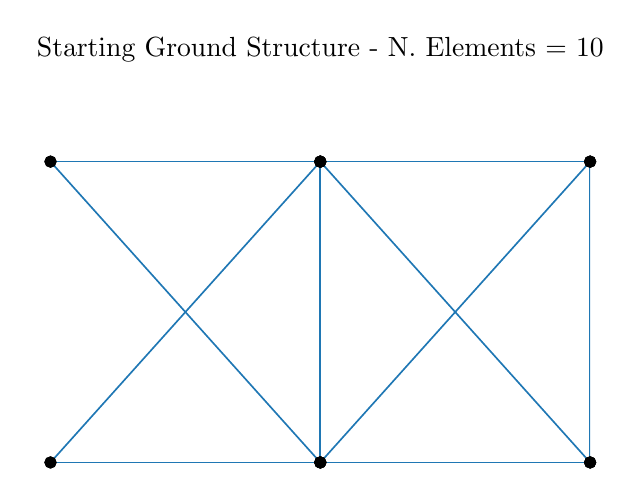
\begin{tikzpicture}

\definecolor{darkgray176}{RGB}{176,176,176}
\definecolor{steelblue31119180}{RGB}{31,119,180}

\begin{axis}[
hide x axis,
hide y axis,
tick align=outside,
tick pos=left,
title={Starting Ground Structure - N. Elements = 10},
x grid style={darkgray176},
xmin=0, xmax=720,
xtick style={color=black},
y grid style={darkgray176},
ymin=-88.258064516129, ymax=448.258064516129,
ytick style={color=black}
]
\path [draw=steelblue31119180, semithick]
(axis cs:0,360)
--(axis cs:360,360);

\path [draw=steelblue31119180, semithick]
(axis cs:360,360)
--(axis cs:720,360);

\path [draw=steelblue31119180, semithick]
(axis cs:0,0)
--(axis cs:360,0);

\path [draw=steelblue31119180, semithick]
(axis cs:360,0)
--(axis cs:720,0);

\path [draw=steelblue31119180, semithick]
(axis cs:360,0)
--(axis cs:360,360);

\path [draw=steelblue31119180, semithick]
(axis cs:720,0)
--(axis cs:720,360);

\path [draw=steelblue31119180, semithick]
(axis cs:360,0)
--(axis cs:0,360);

\path [draw=steelblue31119180, semithick]
(axis cs:0,0)
--(axis cs:360,360);

\path [draw=steelblue31119180, semithick]
(axis cs:720,0)
--(axis cs:360,360);

\path [draw=steelblue31119180, semithick]
(axis cs:360,0)
--(axis cs:720,360);

\addplot [fill=black, mark=*, only marks]
table{%
x  y
0 360
360 360
};
\addplot [fill=black, mark=*, only marks]
table{%
x  y
360 360
720 360
};
\addplot [fill=black, mark=*, only marks]
table{%
x  y
0 0
360 0
};
\addplot [fill=black, mark=*, only marks]
table{%
x  y
360 0
720 0
};
\addplot [fill=black, mark=*, only marks]
table{%
x  y
360 0
360 360
};
\addplot [fill=black, mark=*, only marks]
table{%
x  y
720 0
720 360
};
\addplot [fill=black, mark=*, only marks]
table{%
x  y
360 0
0 360
};
\addplot [fill=black, mark=*, only marks]
table{%
x  y
0 0
360 360
};
\addplot [fill=black, mark=*, only marks]
table{%
x  y
720 0
360 360
};
\addplot [fill=black, mark=*, only marks]
table{%
x  y
360 0
720 360
};
\end{axis}

\end{tikzpicture}
